\chapter{Raccolta e analisi dei requisiti}

\section{Obiettivi della Raccolta dei Requisiti}
% Descrizione: Spiega l'importanza della raccolta dei requisiti e come è stata condotta (interviste, workshop, analisi documentale).
% Stakeholder Coinvolti: Elenca gli stakeholder chiave e il loro ruolo nella definizione dei requisiti.
La raccolta dei requisiti è una fase fondamentale per garantire che il prodotto finale soddisfi gli stakeholder e gli obiettivi prefissati.

L'obiettivo principale di questa fase è identificare, analizzare e documentare le esigenze e le aspettative delle parti interessate, in particolare sono stati individuati tre tipi di requisiti: funzionali, non funzionali e di dominio.
\begin{itemize}
	\item I requisiti funzionali definiscono le funzionalità che il sistema deve offrire, descrivendo come il software interagirà con gli utenti e con altri sistemi.
	\item I requisiti non funzionali, riguardano le qualità del sistema, come le prestazioni, la sicurezza, l'usabilità e la scalabilità.
	\item I requisiti di dominio definiscono le regole di comportamento che il sistema deve applicare.
\end{itemize}

\newpage
\section{Requisiti individuati}
\subsection{Requisiti funzionali}
\begin{itemize}
	\item l'utente può registrare un nuovo account
	\item l'utente può utilizzare un'account da lui registrato per accedere al sistema
	\item l'utente può registrarsi utilizando credenziali di terze pari (es.: google, facebook, …)
	\item l'utente può personalizzare il proprio profilo (non obbligatorio):
	      \begin{itemize}[label={\tiny$\blacksquare$}]
		      \renewcommand{\labelitemi}{\tiny$\blacksquare$}
		      \item aggiungere nome e cognome
		      \item aggiungere una breve bio
		      \item link al proprio sito web
		      \item link ai propri social
	      \end{itemize}
	      \medskip
	\item l'utente può creare un'asta
	      \begin{itemize}[label={\tiny$\blacksquare$}]
		      \item inserisce la foto
		      \item inserisce la descrizione
		      \item inserisce la categoria
		      \item asta all'inglese
		            \begin{itemize}[label={\tiny$-$}]
			            \item il venditore inserisce una base d'asta (visibile a tutti)
			            \item ***(dubbio colloquio 3)*** L'asta include un intervallo di tempo fisso per presentare nuove offerte (di default 1 ora)
			            \item ***(dubbio colloquio 3)*** L'asta include una soglia di rialzo (di default 10€)
		            \end{itemize}
		      \item l'utente può creare un asta al ribasso e inserisce:
		            \begin{itemize}[label={\tiny$-$}]
			            \item un prezzo iniziale
			            \item la durata del timer per il decremento del prezzo (di default 1 ora).
			            \item l'importo per ciascun decremento
			            \item il prezzo minimo segreto (non visibili pubblicamente).
		            \end{itemize}
		      \item l'utente può creare un asta silenziosa
		            \begin{itemize}[label={\tiny$-$}]
			            \item inserisce data e ora di scadenza
			            \item può accettare un'offerta
		            \end{itemize}
	      \end{itemize}

	      \medskip
	\item l'utente può presentare un'offerta (per qualsiasi tipo d'asta) \medskip

	\item l'utente può cercare un'asta per parola chiave
	\item l'utente può filtrare le aste per categoria (tecnologia, giocattoli, …) \medskip

	\item l'utente può visualizzare i dettagli di un'asta
	\item l'utente può visualizzare il profilo del venditore dell'asta \medskip

	\item Visualizzazione storico aste create (in corso e concluse)
	\item Visualizzazione storico a cui hai partecipato (in corso e concluse)
\end{itemize}

\newpage
\subsection{Requisiti non funzionali}
\begin{itemize}
	\item il sistema deve gestire la concorrenza in caso di offerte uguali contemporaneamente:

	      Se, in un'asta all'inglese, più compratori fanno la stessa offerta contemporaneamente, solo uno avrà la meglio.

	      Stesso discorso per un'asta al ribasso, se più compratori decidono di acquistare l'asta a quel prezzo, solo uno avrà la meglio.
\end{itemize}
\begin{enumerate}
	\item {\sffamily \textbf{Usabilità}}:\\
	      L'interfaccia utente deve essere intuitiva e facile da utilizzare, con una chiara visualizzazione delle informazioni relative alle aste e ai profili utenti.

	\item {\sffamily \textbf{Performance}}:\\
	      Il sistema deve gestire in modo efficiente un grande numero di aste e utenti, garantendo tempi di risposta rapidi, specialmente durante la presentazione delle offerte e la gestione dei timer.

	\item {\sffamily \textbf{Scalabilità}}:\\
	      Il sistema deve essere scalabile per supportare un numero crescente di utenti, aste e operazioni contemporanee senza compromettere le prestazioni.

	\item {\sffamily \textbf{Sicurezza}}:\\
	      Gli utenti devono poter registrarsi e autenticarsi in modo sicuro, anche tramite provider di terze parti.

	      Devono essere implementate misure per proteggere le offerte e i dati personali degli utenti.

	\item {\sffamily \textbf{Affidabilità}}:\\
	      Il sistema deve essere altamente disponibile, minimizzando i tempi di inattività.

	      I dati relativi alle aste, alle offerte e ai profili devono essere conservati in modo sicuro e accessibili in qualsiasi momento.
\end{enumerate}

\newpage
\subsection{Requisiti di dominio}
\begin{itemize}
	\item l'email è univoca per ogni account. Non possono esserci più account con una sola mail
	\item un account è sia venditore che compratore
	\item l'utente non può acquistare le aste create da lui stesso
	\item l'asta può essere di diversi tipi: all'inglese, al ribasso, silenziosa:
	      \begin{itemize}[label={\tiny$\blacksquare$}]
		      \item {\sffamily \textbf{Asta all'inglese}}: Un formato in cui le offerte incrementano il prezzo fino alla scadenza del timer, con vincita al miglior offerente.
		      \item {\sffamily \textbf{Asta al ribasso}}: Un formato in cui il prezzo diminuisce con il tempo, e la vendita avviene al primo offerente che accetta il prezzo corrente.
		      \item {\sffamily \textbf{Asta silenziosa}}: Un formato in cui le offerte sono segrete e il venditore sceglie una sola offerta da accettare.
	      \end{itemize}
	\item asta all'inglese:
	      \begin{itemize}[label={\tiny$\blacksquare$}]
		      \item l'offerta può essere presentata a partire dal prezzo corrente.

		            se è la prima offerta può offrire il prezzo base, altrimenti deve presentare un'offerta più alta rispetto al prezzo corrente.

		            Il rialzo dev'essere un multiplo della soglia impostata nell'offerta ***(dubbio colloquio, dev'essere di X alla volta o anche multipli di X?)***

		      \item quando viene presentata un'offerta, il timer viene resettato e il prezzo corrente viene aggiornato
		      \item allo scadere del timer:
		            \begin{itemize}[label={\tiny$-$}]
			            \item l'asta si conclude
			            \item vince l'ultima offerta fatta
			            \item il venditore e gli acquirenti che hanno partecipato all'asta visualizzano una notifica.
		            \end{itemize}
	      \end{itemize}
	\item asta al ribasso:
	      \begin{itemize}[label={\tiny$\blacksquare$}]
		      \item al raggiungimento del timer, il prezzo verrà decrementato dell'importo previsto e il timer riparte
		      \item il prodotto è venduto al primo acquirente che presenta un'offerta
		      \item Se il prezzo raggiunge il prezzo minimo segreto senza offerte, l'asta fallisce e il venditore riceve una notifica. ***(dubbio colloquio l'offerta fallisce al raggiungimento del prezzo minimo oppure fallisce al ribasso successivo al prezzo minimo?)***
	      \end{itemize}
	\item asta silenziosa:
	      \begin{itemize}[label={\tiny$\blacksquare$}]
		      \item le offerte degli utenti sono segrete, non visibili agli altri utenti ma solo al venditore
		      \item il venditore può accettare una sola offerta
		      \item quando il venditore accetta un'offerta, viene inviata una notifica all'acquirente.
	      \end{itemize}

\end{itemize}

\newpage
\section{Modello dei casi d'uso}
\subsection{Tabella}

{
	\setlength{\tabcolsep}{10pt} % Padding orizzontale
	\renewcommand{\arraystretch}{1.5} % Padding verticale

	\begin{tabular}{|l|p{330pt}|}
		\hline
		\textbf{Attore}    & \textbf{Casi d'uso}                                        \\ \hline
		Utente non loggato & \begin{itemize}[leftmargin=15pt]
			                     \setlength{\itemsep}{0pt}  % Riduce lo spazio tra gli elementi della lista
			                     \setlength{\parskip}{0pt}  % Riduce lo spazio tra i paragrafi
			                     \item registrazione con email
			                     \item registrazione con credenziali di terze parti (Google)
			                     \item Accesso al sistema
		                     \end{itemize} \\ \hline
		\makecell{Utente non loggato                                                    \\ (venditore/acquirente)} &
		\begin{itemize}[leftmargin=15pt]
			\setlength{\itemsep}{0pt}  % Riduce lo spazio tra gli elementi della lista
			\setlength{\parskip}{0pt}  % Riduce lo spazio tra i paragrafi
			\item Personalizza il profilo
			\item Visualizza storico
			      \begin{itemize}
				      \item aste create (in corso e concluse)
				      \item a cui hai partecipato (in corso e concluse)
			      \end{itemize}
			\item Ricerca asta per parola chiave
			\item Filtra asta per categoria
			\item Visualizza dettagli di un'asta
			\item Visualizza il profilo del venditore

		\end{itemize}\medskip
		\begin{itemize}[leftmargin=15pt]
			\setlength{\itemsep}{0pt}  % Riduce lo spazio tra gli elementi della lista
			\setlength{\parskip}{0pt}  % Riduce lo spazio tra i paragrafi
			\item Crea asta
			      \begin{itemize}
				      \item all'inglese
				      \item al ribasso
				      \item silenziosa
			      \end{itemize}
		\end{itemize}\medskip
		\begin{itemize}[leftmargin=15pt]
			\setlength{\itemsep}{0pt}  % Riduce lo spazio tra gli elementi della lista
			\setlength{\parskip}{0pt}  % Riduce lo spazio tra i paragrafi
			\item Piazza un'offerta
			      \begin{itemize}
				      \item per l'asta all'inglese
				      \item per l'asta al ribasso
				      \item per l'asta silenziosa
			      \end{itemize}
		\end{itemize}                     \\ \hline
	\end{tabular}
}

\subsection{Descrizioni dettagliate}
\begin{itemize}
	\item \textbf{Registrazione con email.}\\
	      L'utente che desidera registrarsi, può farlo inserendo dati quali: email, nome, cognome e password. I dati inseriti sono soggetti a verifica da parte del sistema (ad esempio: la mail deve essere in un formato valido).

	      Una volta effettuata la registrazione, se questa ha avuto successo, l'utente accede al sistema.

	\item \textbf{Registrazione con credenziali di terze parti (Google).}\\
	      L'utente può registrarsi più utilizzando il proprio account Google. Una volta effettuata la registrazione, se questa ha avuto successo, l'utente accede al sistema.

	\item \textbf{Accesso al sistema.}\\
	      L'utente che ha già effettuato la registrazione in precedenza può accedere al sistema utilizzando la mail con la quale si è registrato e la propria password.

	\item \textbf{Personalizzazione del profilo.}\\
	      Andando nella sezione “Profilo”, l'utente può visualizzare le proprie informazioni e modificarle. Può aggiungere informazioni quali: bio, link al proprio sito personale, link ai social ed area geografica.

	\item \textbf{Visualizzazione storico aste create (in corso e concluse).}\\
	      Andando nella sezione “Storico Aste”, l'utente può visualizzare sia le aste a cui ha preso parte (quelle in corso per cui ha piazzato un'offerta, e quelle concluse) sia le aste che ha creato (in corso e concluse).

	\item \textbf{Ricerca aste per parola chiave.}\\
	      Nella homepage l'utente può selezionare la barra di ricerca e inserire delle parole chiave per filtrare le aste per descrizione, in modo da trovare più velocemente ciò a cui è interessato.

	      \textit{Nota: Se anche il filtraggio per categoria è attivato, la ricerca viene raffinata ulteriormente (parola chiave + categoria).}

	\item \textbf{Filtraggio aste per categoria.}\\
	      Nella homepage l'utente può selezionare dei pulsanti per filtrare le aste visualizzate per categoria.

	\item \textbf{Visualizza dettagli di un'asta.}\\
	      L'utente interessato ad un'asta può cliccarla per accedere alla pagina di dettaglio e visualizzare tutte le informazioni di cui ha bisogno. Da questa schermata è anche possibile fare un'offerta (se l'asta è ancora in corso) e visualizzare il profilo del venditore.

	\item \textbf{Visualizza il profilo del venditore.}\\
	      L'utente che sta visualizzando un'asta può cliccare sul nome del venditore per visualizzare la pagina profilo del venditore.

	\item \textbf{Creare asta all'inglese.}\\
	      Dalla schermata home, l'utente clicca sul pulsante “Crea Asta”, poi clicca sul pulsante "Asta all'inglese". Viene visualizzata una nuova schermata in cui deve inserire tutte le informazioni necessarie tra cui: immagine, descrizione, categoria, base d'asta, soglia di rialzo e il timer.

	\item \textbf{Creare asta al ribasso.}\\
	      Dalla schermata home, l'utente clicca sul pulsante “Crea Asta”, poi clicca sul pulsante "Asta al ribasso". Viene visualizzata una nuova schermata in cui deve inserire tutte le informazioni necessarie tra cui: immagine, descrizione, categoria, prezzo iniziale, prezzo minimo, importo di cui decrementare, timer prima di un decremento.

	\item \textbf{Creare asta silenziosa.}\\
	      Dalla schermata home, l'utente clicca sul pulsante “Crea Asta”, poi clicca sul pulsante "Asta silenziosa". Viene visualizzata una nuova schermata in cui deve inserire tutte le informazioni necessarie tra cui: immagine, descrizione, categoria, scadenza.

	\item \textbf{Piazzare un'offerta per l'asta all'inglese.}\\
	      L'utente che si trova sulla schermata di un'asta all'inglese inserisce l'importo dell'offerta che vuole piazzare, poi clicca sul pulsante "conferma offerta".

	\item \textbf{Piazzare un'offerta per l'asta al ribasso.}\\
	      L'utente che si trova sulla schermata di un'asta al ribasso può cliccare il pulsante “Acquista” ed aggiudicarsi automaticamente l'asta. Dopo quest'operazione il sistema mostra una notifica che informa l'utente dell'esito dell'asta.

	\item \textbf{Piazzare un'offerta per l'asta silenziosa.}\\
	      L'utente che si trova sulla schermata di un'asta silenziosa può inserire un'offerta e cliccare sul pulsante "conferma offerta" per inviare l'offerta.
\end{itemize}

\newpage
\subsection{Diagrammi}
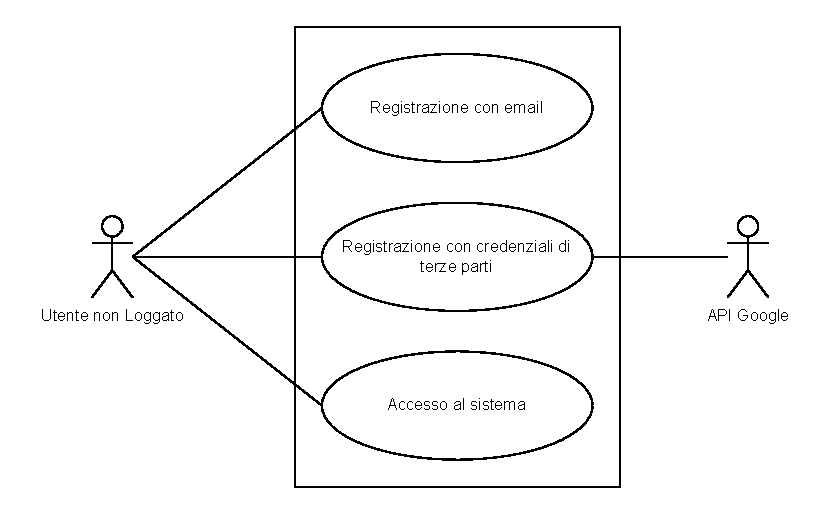
\includegraphics[width=.7\textwidth]{images/utente_non_loggato_use_case_diagram.pdf}

\newpage
\section{Tabelle di Cockburn}
\subsection{Creazione asta silenziosa}
\begin{table}[H]
	\renewcommand{\arraystretch}{1.3}
	\begin{tabularx}{\linewidth}{|p{120pt}|p{40pt}|X|X|}
		\hline \rowcolor[HTML]{DCDCDC}
		\textbf{\large\sffamily Use Case {\ttfamily \#}01} & \multicolumn{3}{p{367pt}|}{\textbf{\large\sffamily Creazione asta silenziosa}}                                                                                                                                                                     \\
		\hline Goal in Context                             & \multicolumn{3}{p{367pt}|}{L'utente vuole creare un'asta silenziosa.}                                                                                                                                                                              \\
		\hline Preconditions                               & \multicolumn{3}{p{367pt}|}{L'utente deve aver effettuato l'accesso.}                                                                                                                                                                               \\
		\hline Success End Conditions                      & \multicolumn{3}{p{367pt}|}{L'utente crea correttamente l'asta silenziosa che poi sarà accessibile agli altri  utenti.}                                                                                                                             \\

		\hline \rowcolor[HTML]{DCDCDC}
		\multirow{1}{*}{}{\textbf{\sffamily Description}}  & \textbf{\sffamily Step}                                                                                                & \textbf{\sffamily User Action}                                   & \textbf{\sffamily System}                              \\
		\cline{2-4}                                        & 1                                                                                                                      & Dal mockup "Homepage" preme il pulsante "Carica Asta".           &                                                        \\
		\cline{2-4}                                        & 2                                                                                                                      &                                                                  & Mostra il mockup "Carica Asta" con 3 possibili scelte. \\
		\cline{2-4}                                        & 3                                                                                                                      & Seleziona il pulsante "Crea Asta silenziosa"                     &                                                        \\
		\cline{2-4}                                        & 4                                                                                                                      &                                                                  & \makecell{Mostra il mockup                             \\ "Creazione Asta silenziosa" }          \\
		\cline{2-4}                                        & 5                                                                                                                      & Inserisce tutti i dati necessari e preme il pulsante "Crea Asta" &                                                        \\
		\cline{2-4}                                        & 6                                                                                                                      &                                                                  & \makecell{Mostra un popup con l'esito                  \\ della creazione dell'asta \\ e torna al mockup "Homepage"} \\

		\hline \rowcolor[HTML]{DCDCDC}
		\multirow{1}{*}{}{\textbf{\sffamily Extensions}}   & \textbf{\sffamily Step}                                                                                                & \textbf{\sffamily User Action}                                   & \textbf{\sffamily System}                              \\
		\hline
		\multirow{1}{*}{}{Dati mancanti o non corretti}    & 5.a                                                                                                                    &                                                                  & Mostra un popup di errore                              \\
		\cline{2-4}                                        & 5.b                                                                                                                    & \makecell{Visualizza il popup e riprova                                                                                   \\ l'inserimento dei dati}  &                                                        \\

		\hline
	\end{tabularx}
\end{table}

\newpage
\subsection{Offerta asta silenziosa}
\begin{table}[H]
	\renewcommand{\arraystretch}{1.3}
	\begin{tabularx}{\linewidth}{|p{120pt}|p{40pt}|X|X|}
		\hline \rowcolor[HTML]{DCDCDC}
		\textbf{\large\sffamily Use Case {\ttfamily \#}01} & \multicolumn{3}{p{367pt}|}{\textbf{\large\sffamily Offerta asta silenziosa}}                                                              \\
		\hline Goal in Context                             & \multicolumn{3}{p{367pt}|}{ INSERISCI TESTO }                                                                                             \\
		\hline Preconditions                               & \multicolumn{3}{p{367pt}|}{ INSERISCI TESTO }                                                                                             \\
		\hline Success End Conditions                      & \multicolumn{3}{p{367pt}|}{ INSERISCI TESTO }                                                                                             \\

		\hline \rowcolor[HTML]{DCDCDC}
		\multirow{1}{*}{}{\textbf{\sffamily Description}}  & \textbf{\sffamily Step}                                                      & \textbf{\sffamily User Action} & \textbf{\sffamily System} \\
		\cline{2-4}                                        &                                                                              &                                &                           \\

		\hline \rowcolor[HTML]{DCDCDC}
		\multirow{1}{*}{}{\textbf{\sffamily Extensions}}   & \textbf{\sffamily Step}                                                      & \textbf{\sffamily User Action} & \textbf{\sffamily System} \\
		\cline{2-4}                                        &                                                                              &                                &                           \\

		\hline
	\end{tabularx}
\end{table}

\newpage
\subsection{Aggiungere link social}
\begin{table}[H]
	\renewcommand{\arraystretch}{1.3}
	\begin{tabularx}{\linewidth}{|p{120pt}|p{40pt}|X|X|}
		\hline \rowcolor[HTML]{DCDCDC}
		\textbf{\large\sffamily Use Case {\ttfamily \#}01} & \multicolumn{3}{p{367pt}|}{\textbf{\large\sffamily Aggiungere link social}}                                                              \\
		\hline Goal in Context                             & \multicolumn{3}{p{367pt}|}{ INSERISCI TESTO }                                                                                            \\
		\hline Preconditions                               & \multicolumn{3}{p{367pt}|}{ INSERISCI TESTO }                                                                                            \\
		\hline Success End Conditions                      & \multicolumn{3}{p{367pt}|}{ INSERISCI TESTO }                                                                                            \\

		\hline \rowcolor[HTML]{DCDCDC}
		\multirow{1}{*}{}{\textbf{\sffamily Description}}  & \textbf{\sffamily Step}                                                     & \textbf{\sffamily User Action} & \textbf{\sffamily System} \\
		\cline{2-4}                                        &                                                                             &                                &                           \\

		\hline \rowcolor[HTML]{DCDCDC}
		\multirow{1}{*}{}{\textbf{\sffamily Extensions}}   & \textbf{\sffamily Step}                                                     & \textbf{\sffamily User Action} & \textbf{\sffamily System} \\
		\cline{2-4}                                        &                                                                             &                                &                           \\

		\hline
	\end{tabularx}
\end{table}

\newpage
\subsection{Visualizzazione profilo venditore}
\begin{table}[H]
	\renewcommand{\arraystretch}{1.3}
	\begin{tabularx}{\linewidth}{|p{120pt}|p{40pt}|X|X|}
		\hline \rowcolor[HTML]{DCDCDC}
		\textbf{\large\sffamily Use Case {\ttfamily \#}01} & \multicolumn{3}{p{367pt}|}{\textbf{\large\sffamily Visualizzazione profilo venditore}}                                                              \\
		\hline Goal in Context                             & \multicolumn{3}{p{367pt}|}{ INSERISCI TESTO }                                                                                                       \\
		\hline Preconditions                               & \multicolumn{3}{p{367pt}|}{ INSERISCI TESTO }                                                                                                       \\
		\hline Success End Conditions                      & \multicolumn{3}{p{367pt}|}{ INSERISCI TESTO }                                                                                                       \\

		\hline \rowcolor[HTML]{DCDCDC}
		\multirow{1}{*}{}{\textbf{\sffamily Description}}  & \textbf{\sffamily Step}                                                                & \textbf{\sffamily User Action} & \textbf{\sffamily System} \\
		\cline{2-4}                                        &                                                                                        &                                &                           \\

		\hline \rowcolor[HTML]{DCDCDC}
		\multirow{1}{*}{}{\textbf{\sffamily Extensions}}   & \textbf{\sffamily Step}                                                                & \textbf{\sffamily User Action} & \textbf{\sffamily System} \\
		\cline{2-4}                                        &                                                                                        &                                &                           \\

		\hline
	\end{tabularx}
\end{table}

\newpage

\section{Mockup del Software}